\section{Sikkerhed}

\paragraph{Spørgsmål}
Redegøre for relevante sikkerhedsmæssige udfordringer ved implementeringen og brugen af en webløsning.	Vis hvordan man kan implementere authorisation og authentication i en webløsning.	Redegøre for hvordan man kan optimere performance for en webapplikation. Redegøre for hvordan man kan publicere webløsninger til driftsmiljøer, her under også cloud baseret hosting.

\subsection{Sikkerhed}
Sikkerhedsmæssige udfordringer i forbindelse med webløsninger. Generelt skal der bruges HTTPS, som kræver et certifikat. \textit{Let's Encrypt} udsteder gratis.

\begin{multicols}{2}
\subsubsection{Autentifikation} 
Bruges til at bestemme brugerens identitet. 

\begin{enumerate}
	\item SALT $\Rightarrow$ HASH
	\item Udsted JWT
\end{enumerate}

\subsubsection{Autorisation} 
Bestemmer hvad en bruger har rettigheder til.

\begin{itemize}
	\item Claim i JWT
	\item Valideres med server-side secret
\end{itemize}
\end{multicols}

Her kan \textit{Basic Autentifikation} bruges, men HTTPS bliver meget vigtigere.

\subsubsection{JSON Web Tokens}
Standard for Bearer tokens.

\begin{multicols}{2}
	\paragraph{Fordele}

	\begin{itemize}
		\item Stateless server
		\item Behøver ikke at tilgå password
		\item CSRF ikke et problem
	\end{itemize}

	\paragraph{Ulemper}
	
	\begin{itemize}
		\item Kan ikke invalideres
		\item Token kan interceptes
	\end{itemize}
\end{multicols}

\subsubsection{Cross-Origin Ressource Sharing}
Med CORS er det muligt at tillade andre servere at kald ens egen og på samme tid afvise andre. En ressource er på ''same origin'' hvis den har samme: scheme, host og port. Figur~\ref{fig:cors-same-origin} viser forskellene.

\begin{figure}[h]
	\centering
	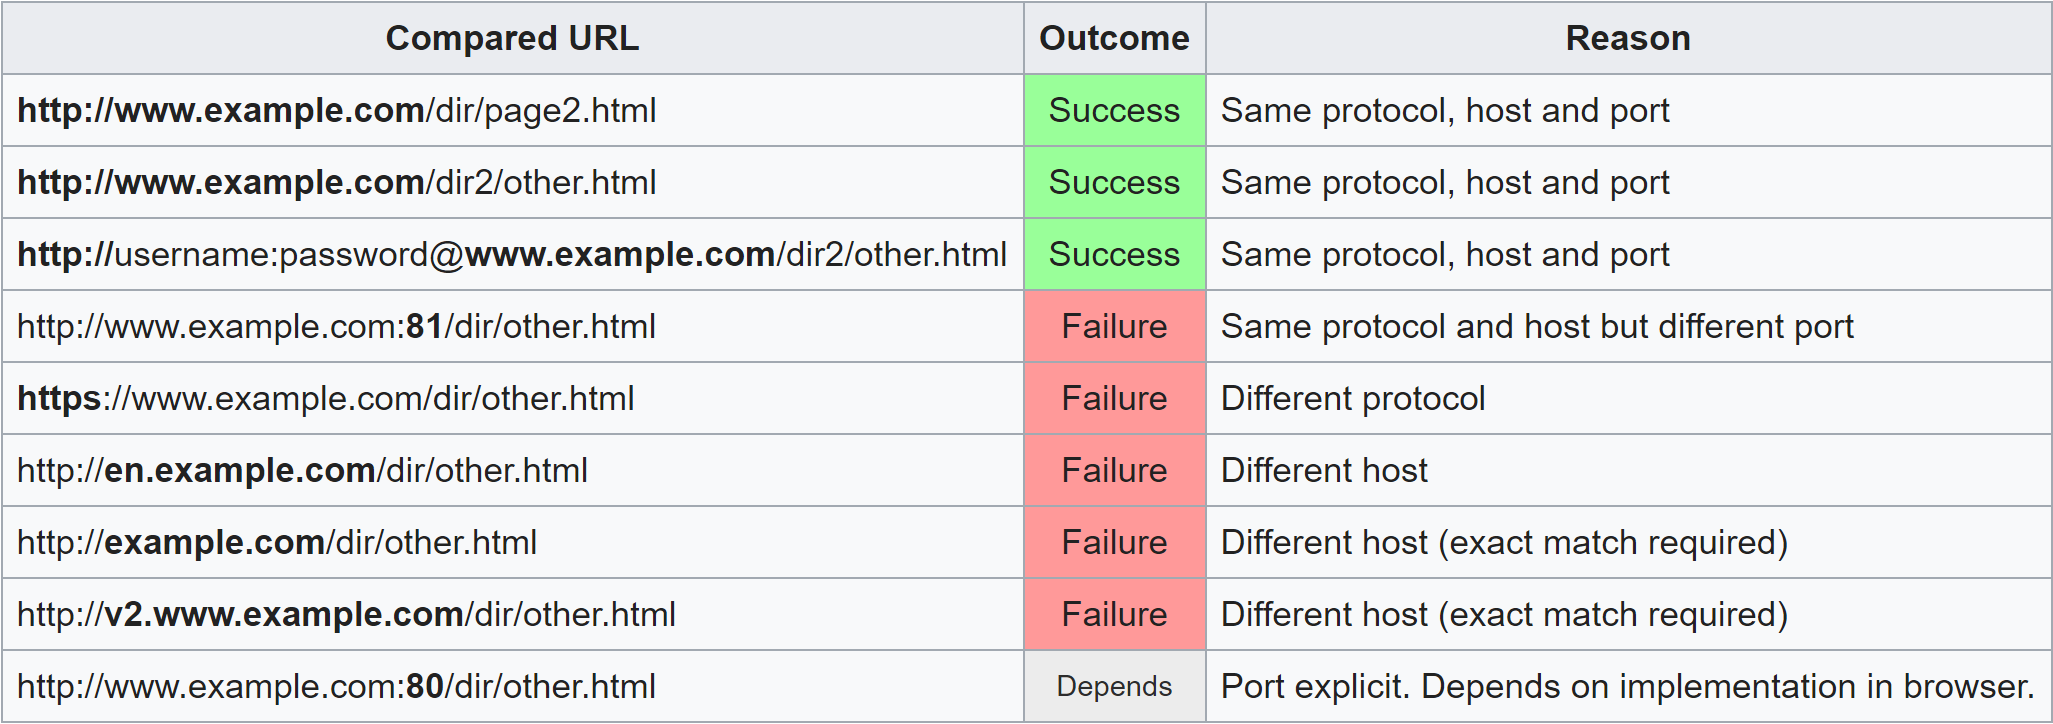
\includegraphics[width=\linewidth]{figs/spm6/cors-same-origin}
	\caption{Same origin defineret.}
	\label{fig:cors-same-origin}
\end{figure}


\subsection{OWASP}
Mest gængse sikkerhedsfejl fra OWASP 2013.

\begin{multicols}{2}
	\begin{itemize}
		\item A1 - Injection
		\item A2 - Broken Authentication and Session
		\item A3 - Cross-Site Scripting (XSS)
		\item A4 - Insecure Direct Object References
		\item A5 - Security Misconfiguration
		\item A6 - Sensitive Data Exposure
		\item A7 - Missing Function Level Access
		\item A8 - Cross-Site Request Forgery (CSRF)
		\item A9 - Using Known Vulnerabilites
		\item A10 - Unvalidated Redirects and Forwards
	\end{itemize}
\end{multicols}

\subsection{Performance optimering}
For at optimere siden kan flere ting gøres: 

\begin{multicols}{2}
\begin{itemize}
	\item Brug CDN
	\item Minify scripts
	\item Cache data aktivt
	\item Indlæs CSS først og JS til sidst
	\item Skaler billeder til skærmstørrelse
	\item Tracking og analytics til sidst (Firefox)
	\item Brug aync ved kald ud af appen
	\item Bedre server og båndbredde
	\item Servere i flere regioner
\end{itemize}
\end{multicols}

\subsection{Drift}
Følgende tjenester kan bruges til at hosting: 

\begin{multicols}{2}
	\begin{itemize}
		\item Digital Ocean
		\item Scaleway
		\item Google Cloud
		\item Heroku
		\item Microsoft Azure
		\item mLab
	\end{itemize}
\end{multicols}

\subsubsection{Teknologier}
For at køre systemerne i disse hosting miljøer kan følgende teknologier anvendes:

\begin{itemize}
	\item Docker
	\item Kubernetes
	\item OpenShift
	\item Microsoft Service Fabric
\end{itemize}
